\section{Experimental Results}
\label{ExpResult}

\subsection{Validity of Pattern Strategy}
\label{validPattern}

Before \emph{PPISnowball} system starts to run, it is essential to make sure whether our pattern strategies are meaningful. How to define "meaningfulness"? We believe that a qualified pattern strategy should somewhat reveal the rules of language usage, such as scale-freeness\cite{DBLP:journals/advcs/Corominas-MurtraVS09}. We check the distribution of patterns by their occurrence number in terms of Shallow Linguistic Pattern, Tri-Branch Part-Of-Speech(POS) Tree Pattern and Tri-Branch Dependency Tree Pattern respectively. All three patterns accord with scale-free distribution, with coefficient 2.683 (Figure \ref{fig:valFig}A), 2.454 (Figure \ref{fig:valFig}B), 2.519 accordingly (Figure \ref{fig:valFig}C). In sum, the pattern strategies we proposed (Section \ref{GenPatterns}) are appropriate for \emph{PPISnowball} process.

\begin{flushleft}
\begin{figure}
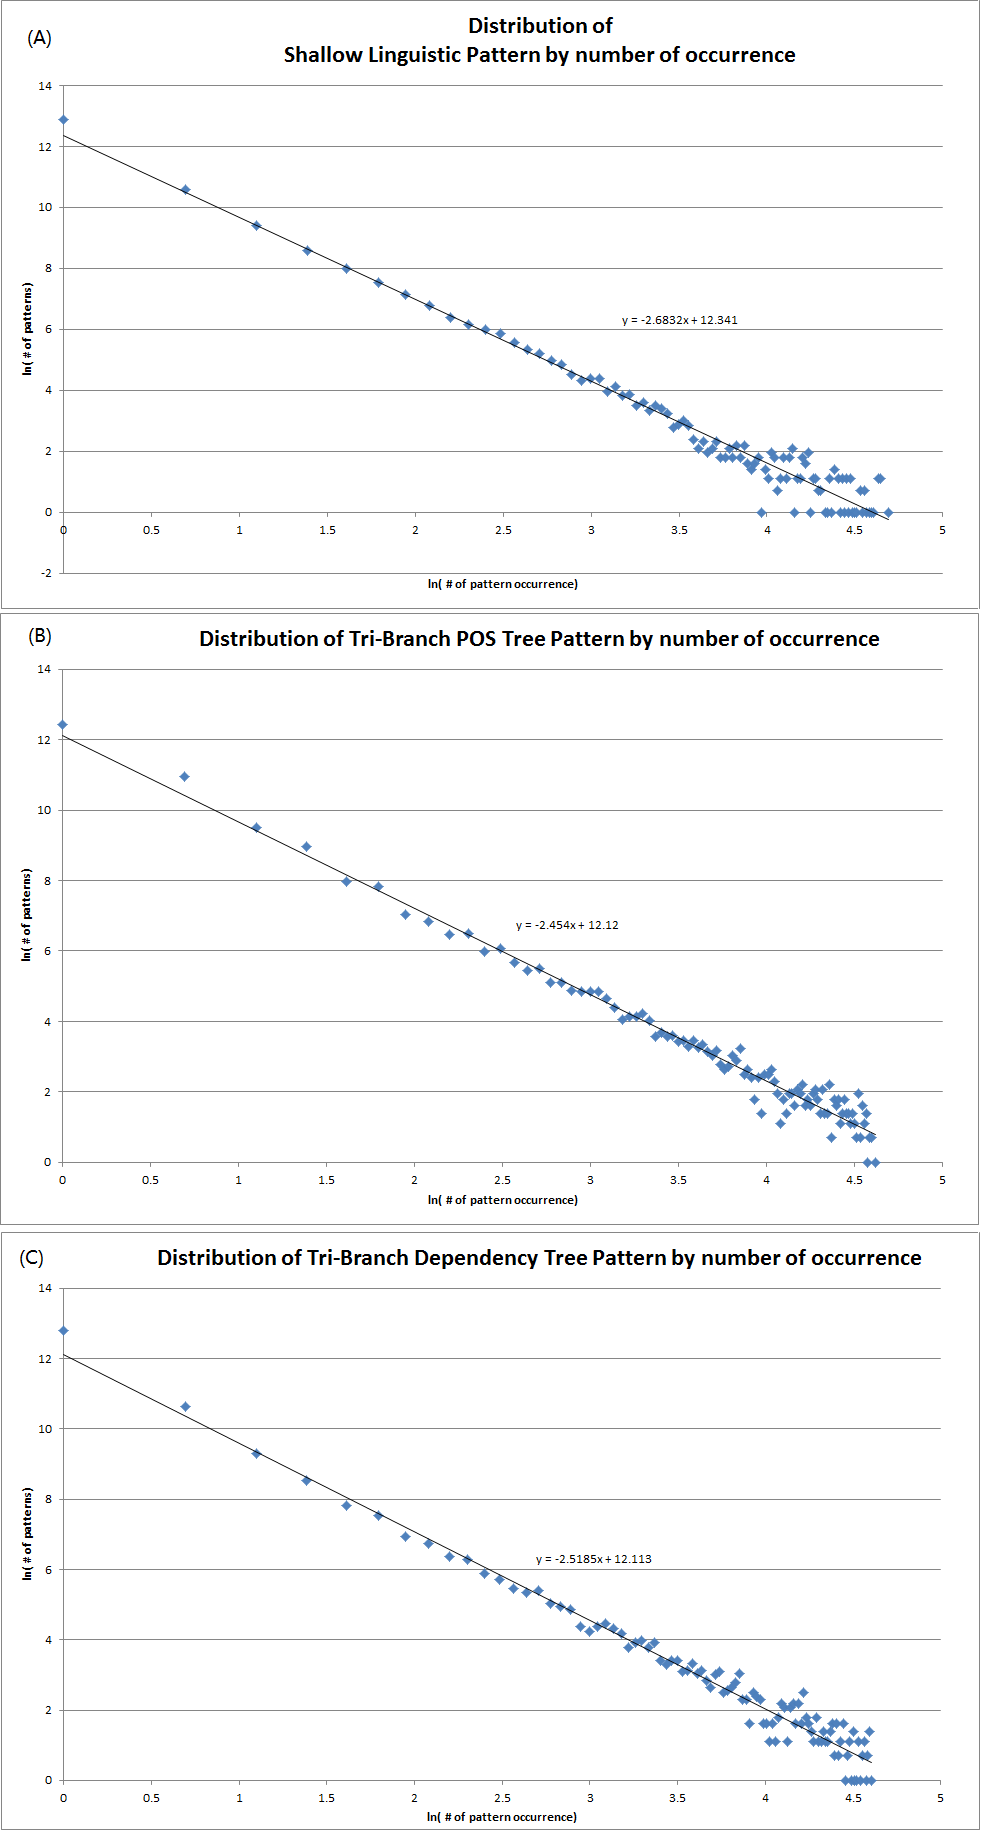
\includegraphics[width=90mm]{fig/figure8.png}
\caption{test}
\label{fig:valFig}
\end{figure}
\end{flushleft}

\subsection{Dataset}
\label{exp:Dataset}

We use a well-known human PPI databases BioGRID\cite{DBLP:journals/nar/StarkBRBBT06} (http://www.thebiogrid.org/) for experiment, the version of BioGRID is 3.1.88. In this case, the dictionary of protein names mentioned by BioGRID contains 172,801 protein names overall, including both official name and alias. Besides, the protein interaction word dictionary is provided by the work of Temkin and Gilder \cite{Temkin03Interactionword}, which is frequently used to describe PPI relationship in biological literatures. BioGRID records 344,958 distinctive positive protein tuples, mentioned in the scope of 31,062 PUBMED articles.

For the sake of convenience and availability, here we only use abstract of articles for the dataset of \emph{PPISnowball} system. As 39 out of 31,062 of articles have no abstract, among the remaining 31,023 abstracts, there are only 35,986 triplets mentioned in 10,449 sentences, for it is possible for a sentence to contain multiple triplets. Among 35,986 triplets, there are only 4,597 distinctive protein tuples, which serve as the theoretical maximum result set of \emph{PPISnowball} system, in other words, the denominator of \emph{recall}. By contrast, the overall 344,958 positive protein tuples play the role of corpora containing all positive tuples, we just ignore the tiny possibility that there might exist leftover positive protein tuples not included in these 344,958 positive tuple set \cite{DBLP:journals/bioinformatics/ChowdharyZL09}.

We manually select some sentences which contain at least one triplet. For one specific triplet in a sentence, we classify it to be positive if the two corresponding proteins are logistically associated via the interaction represented by interaction word, otherwise negative. Among those manually-tagged triplets, we select 500 positive protein tuples and 500 negative respectively. Only a fraction of each kind of tuples would be selected as the input to \emph{PPISnowball} system.

\subsection{Choice of Parameters}
\label{exp:param}

\begin{table}
\begin{center}
\begin{tabular}{||l|l|l||}
\hline
Parameter &  Value  & Description \\
\hline
$\mathcal {T}_{sup}$ & 5 & minimum pattern support \\
$\mathcal {T}_{sim}$ &  0.6 &  minimum similarity for augmentation \\
$\bbbeta$ & 0.8 & Dacay Factor for augmented patterns  \\
$\mathcal {T}_{t}$ & 0.6 & minimum tuple confidence \\
$W_{updt}$ & 0.5 & pattern learning rate \\
$W_{own}$ & 0.5 & pattern augmentation rate \\
$W_{pos}$ & 1.0 & weight for positive triplets \\
$W_{neg}$ & 2.0 & weight for negative triplets \\ $W_{unkn}$ & 0.1 & weight for unknown triplets (Section \ref{EvalPatterns}) \\ \hline
\end{tabular}
\end{center}
\end{table}

\subsection{Evaluation Metrics}
\label{exp:EvalMet}

We use \emph{precision}, \emph{recall}, \emph{F-score}, \emph{specificity}, \emph{accuracy} as our metrics to evaluate the performances of \emph{PPISnowball} system. These metrics are defined as follows:

\begin{equation}
\begin{aligned}
Precision &= TP/(TP+FP)  \nonumber \\
Recall &= TP/(TP+FN)  \nonumber \\
F-score &= \frac{2*Precision*Recall}{Precision+Recall}
\end{aligned}
\end{equation}

\emph{where TP(True Positive) is the number of positive tuples correctly classified as positive; FP(False Positive) is the number of negative tuples mistakenly classified as positive; TN(True Negative) is the number of negative tuples correctly classified as negative; and FN(False Negative) is the number of positive tuples mistakenly classified as negative.} \\

In all, the \emph{selectiveness} of \emph{PPISnowball} system can be weighed by \emph{precision}, and the \emph{coverage} can be measured by \emph{recall}. Besides, \emph{F-score} is the harmonic mean of \emph{precision} and \emph{recall}, showing a comprehensive judgement of both \emph{selectiveness} and \emph{coverage}.

\subsection{Results of different patterns and kernels}
\label{exp:ResultsByPtnKnl}

\begin{table}[htbp]
 \centering
 \small
 \begin{threeparttable}
 \caption{\label{tab:results}Results of \emph{PPISnowball} using different patterns and kernels}
  \begin{tabular}{lccc}
  \toprule
           &   Precision &   Recall &  F-score  \\

  \midrule
  SL            &     &     &  \\
  POS-rigid     &     &     &  \\
  POS-ST        &     &     &  \\
  POS-SST       &     &     &  \\
  POS-SpT       &     &     &  \\
  Dep-rigid     &     &     &  \\
  Dep-ST        &     &     &  \\
  Dep-SST       &     &     &  \\
  Dep-SpT       &     &     &  \\

  \bottomrule
  \end{tabular}

  Note: The figures shown are all in percent.
 \end{threeparttable}
\end{table}

